% ----------------------------------------------------------
% PARTE
% ----------------------------------------------------------
\part{Resultados}
% ----------------------------------------------------------

\section{Kaggle}

Kaggle é uma plataforma criada em 2010 que reune ferramentas e estudos sobre modelagem preditiva. Também viabiliza competições de temas relacionados a análise preditiva. Com o intuito de compartilhar conhecimento, qualquer interessado pode acessar dados de empresas para aplicar estudos ou gerar novos modelos. Além disso, o Kaggle também tem sido usado como uma forma de recrutar cientistas de dados. 


\subsection{Loan Club}

A Loan Club é um marketplace de créditos online. Trata-se de uma plataforma que reune pessoas que gostaria de realizar um empréstimo e outras que possuem um capital a investir. Em geral, são empréstimos pessoas, de negócios ou para procedimentos médicos. A proposta é oferecer um serviço de fácil acesso via dispositivos mobiles a taxa baixas, além de garantir um retorno que se ajuste a expectativa do investidor. Dessa forma, operam de forma menos burocrática do que um banco, mas assumindo os riscos de uma instituição financeira.


\section{Tecnologias}

\subsection{Scikit Learn}

O scikit é um framework desenvolvido em Python voltado para data science. Possui implementação de diversos algoritmos e de ferramentas que auxiliam desde a análise dos dados até na execução de tarefas como clusterização e classificação até a execução dos algoritmos de machine learning. Possui integrações com programas visuais (como será mostrado a seguir). Já são mais de 30 contribuidores ativos.


\subsection{Apache Spark}

O Apache Spark é uma ferramenta que resolve um problema relacionado a escalabilidade da execução de algoritmos de machine learning. Os 3 algoritmos estudos (em especial o Kmédias) possui uma carga de contas alto. Para bases grandes, aspecto relevante quando se trata de Big Data, o scikit não é capaz de executar em tempo hábil. O Apache Spark, por outro lado, oferece uma solução robusta para a execução dos algoritmos de machine learning. Embora seja possível configurá-lo para que os algortimos sejam executados em tempo real com alimentação contínua de dados, tal abordagem não será contemplada por não se tratar do foco do estudo.

\section{Algoritmos}

\subsection{Preparação da base}

Como uma base de uma empresa, o Loan Club apresenta diversos problemas como:

- Missing values
Ocorre quando uma informação não consta na base. Esse fato influencia na conclusão de uma análise porque é necessário verificar a natureza da informação. Elas são oriundas desde problemas ao guardar a informação (como erro humano, falta de informação ou em decorrência de algum problema ou inconsistência no sistema que armazenou). Para os algortimos, é necessário que algum valor seja colocado para a realização das cálculos dos algoritmos. Nessas situações, existem abordagens diferentes, como subustituição por um valor padrão que faça sentido. Em alguns casos, são usados valores considerado neutros como 0, média ou moda das observações. Contido, é evidente que cada uma dessas técnicas enviesa e modifica o resultado. Para essa situação, neste estudo, desprezamos as informações que possuiam altas ocorrências de missing values.

- Necessidade de tratamentos de dados
Foram realizados 3 transformações: normalização de dados para o k médias, tratamento de dados de texto para valores (completar) e remoção das variáveis categóricas.

\subsection{K Médias}

PS: perguntar sobre normalização

No diagrama de Voronoi é possível ter uma visualização espacial da distribuição dos registros, bem como os centróides.

\begin{figure}[!ht]
\caption{Visualização dos pontos no diagrama de Voronoi }
\centerline{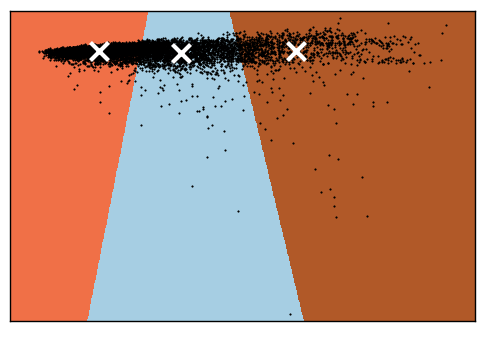
\includegraphics[width=0.5\textwidth]{img/voronoi}}
\fonte{Gerado a partir do script}
\end{figure}

 Para isso, foi necessário realizar uma operação de redução de dimensionalidade de veriáveis para 2 features. Neste estudo, aplicamos a construção do diagrama para 8000 registros.


Também é possível fazer uma análise para verificar a quantidade de clusters ideal para a amostragem.

\begin{figure}[!ht]
\caption{Analise para 2 clusters }
\centerline{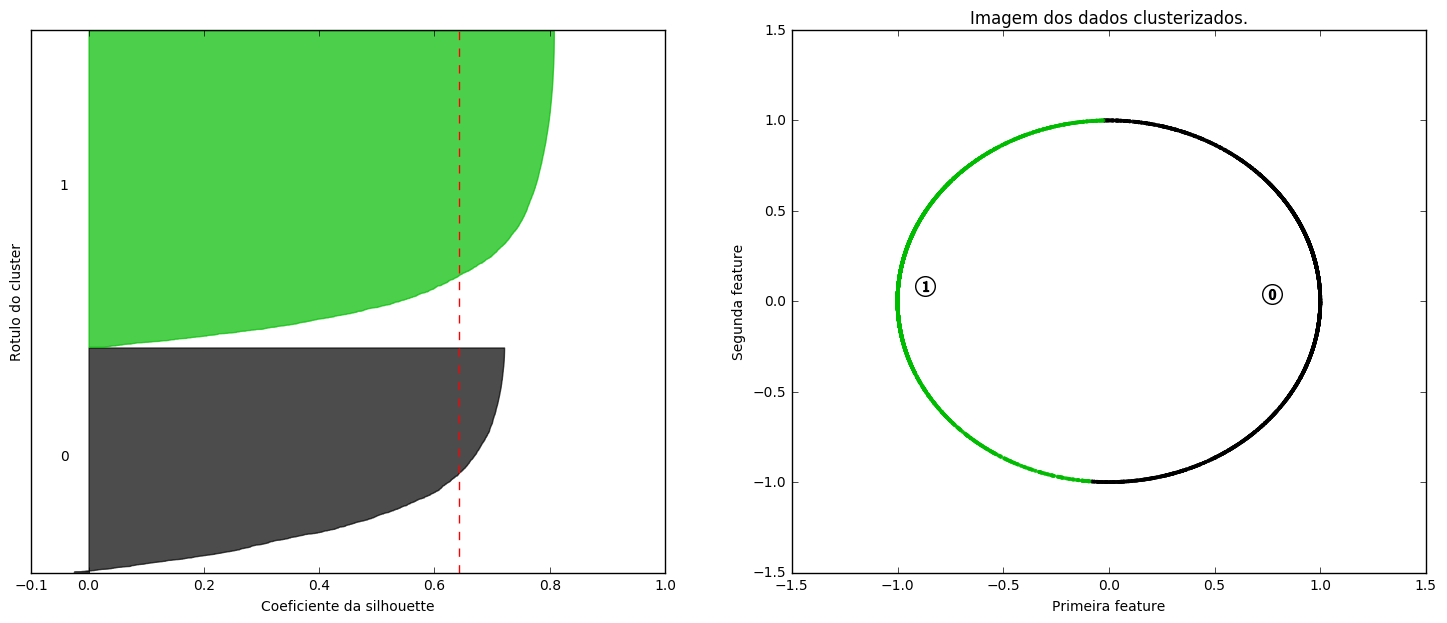
\includegraphics[width=.8\textwidth]{img/silhoute2}}
\fonte{Gerado a partir do script}
\end{figure}

Para a divisão em 2 clusters, foi obtida a nota 0,5516

\begin{figure}[!ht]
\caption{Analise dos 3 clusters }
\centerline{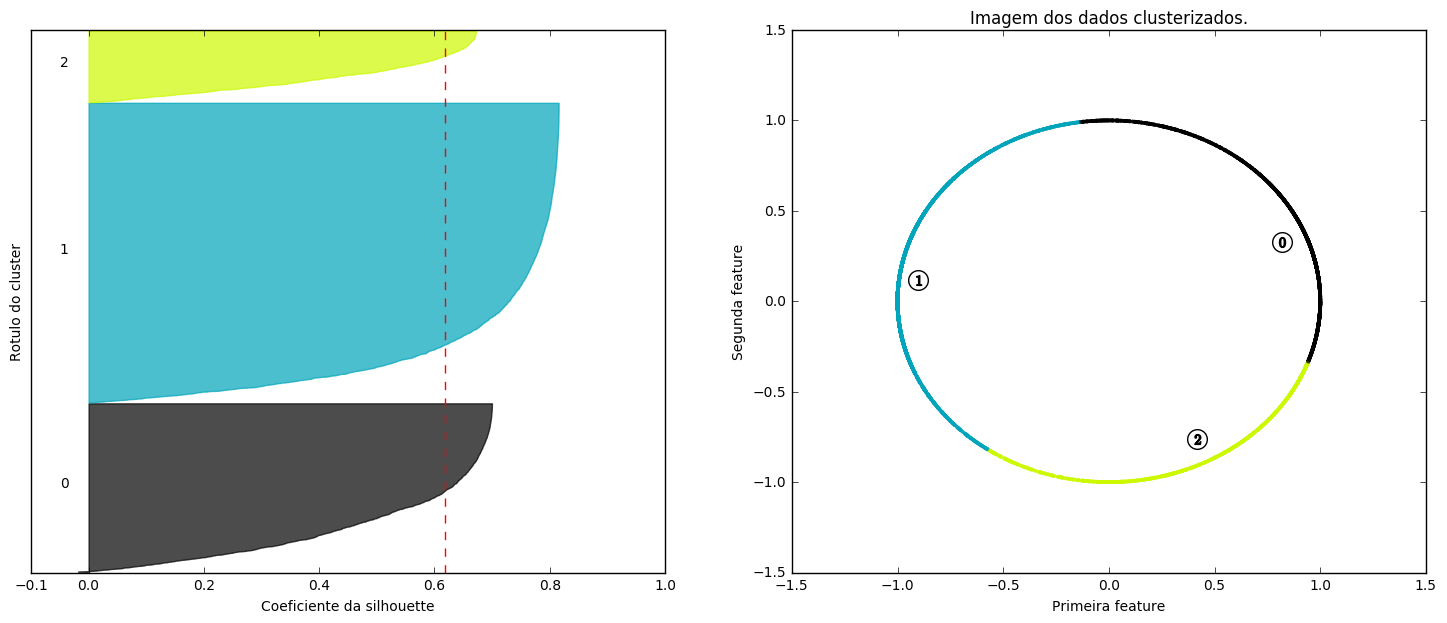
\includegraphics[width=.8\textwidth]{img/silhoute3}}
\fonte{Gerado a partir do script}
\end{figure}

Para a divisão em 3 clusters, foi obtida a nota 0,4463

\begin{figure}[!ht]
\caption{Analise dos 4 clusters }
\centerline{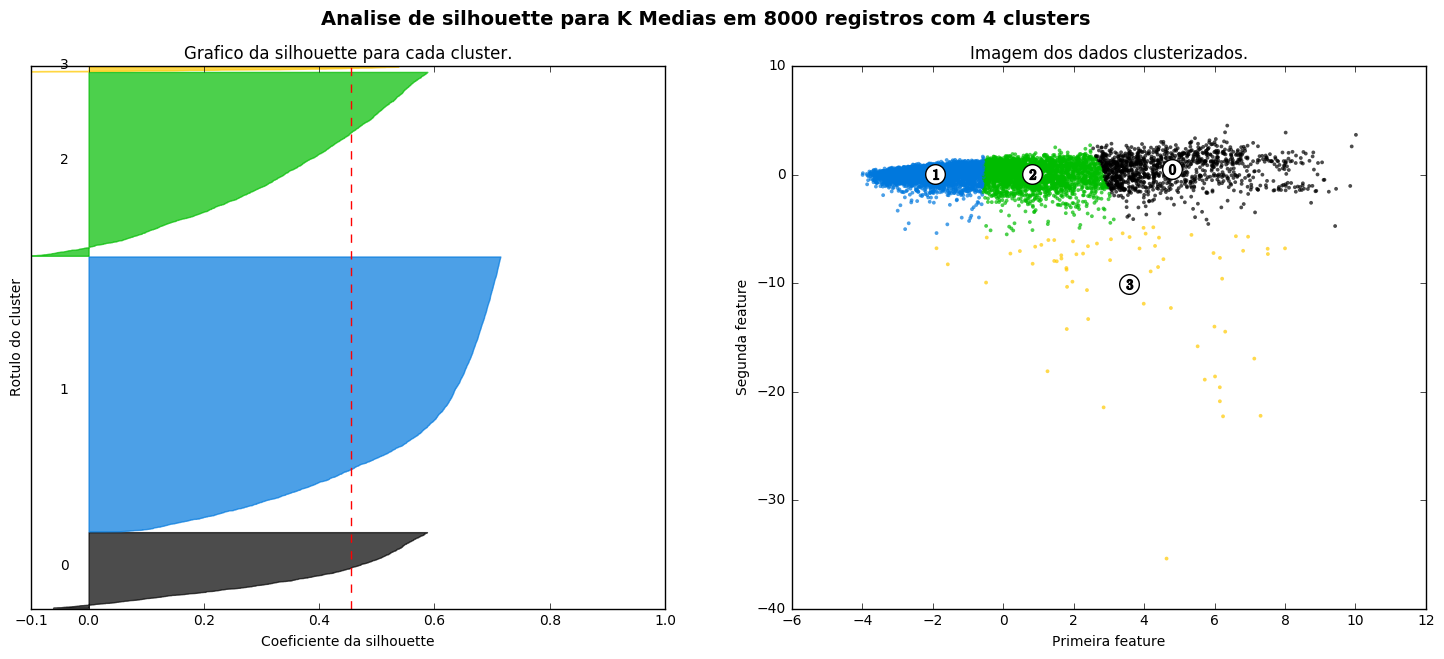
\includegraphics[width=.8\textwidth]{img/silhoute4}}
\fonte{Gerado a partir do script}
\end{figure}

Para a divisão em 4 clusters, foi obtida a nota 0,4559

\begin{figure}[!ht]
\caption{Analise dos 5 clusters }
\centerline{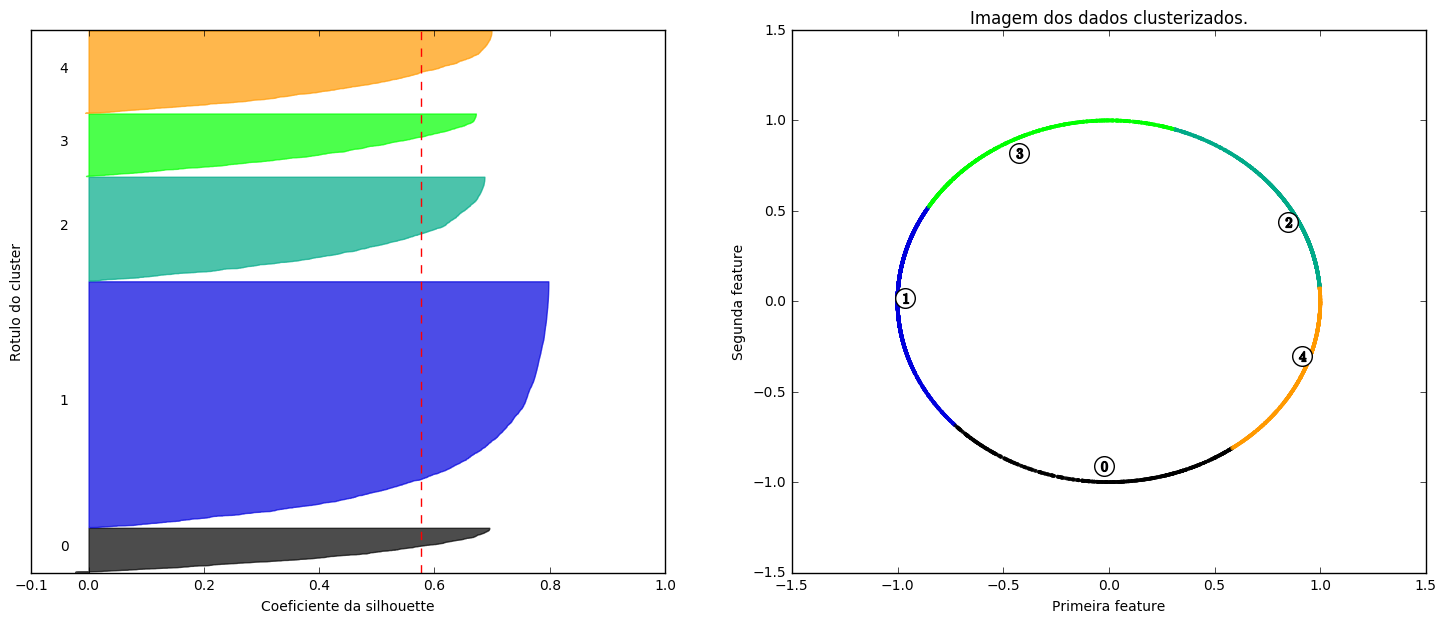
\includegraphics[width=.8\textwidth]{img/silhoute5}}
\fonte{Gerado a partir do script}
\end{figure}

Para a divisão em 5 clusters, foi obtida a nota 0,4032

Podemos notar uma tendência do score cair. Contudo, maior o score, melhor. Dessa forma, há um indício de que uma boa clusterização seja com 2 centróides.



\subsection{Regressão Logística}


Também conhecida como matriz de erros, a confusion matrix é uma representação visual dos erros ocorridos durante o processamento do algoritmo. As linhas representam a classe que o dado pertence e a coluna representa a classificação gerada durante o processo. Quando um registro não está dentro da diagonal principal, significa que o algoritmo fez uma classificação diferente do que foi esperado.

\begin{figure}[!ht]
\caption{Confusion Matrix}
\centerline{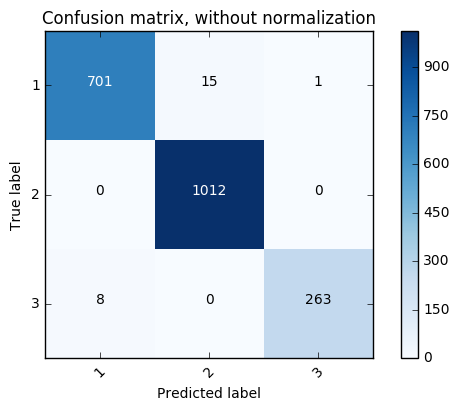
\includegraphics[width=.7\textwidth]{img/confusionMatrix}}
\fonte{Gerado a partir do script}
\end{figure}


Para o caso do Loan Club, podemos notar que a função gerada pela regressão logística possui um indíce de acurácia alto.

\subsection{Random Forest}

A árvore de classificação para 3 clusters é essa

\begin{figure}[!ht]
\caption{Estrutura da arvore de decisao}
\centerline{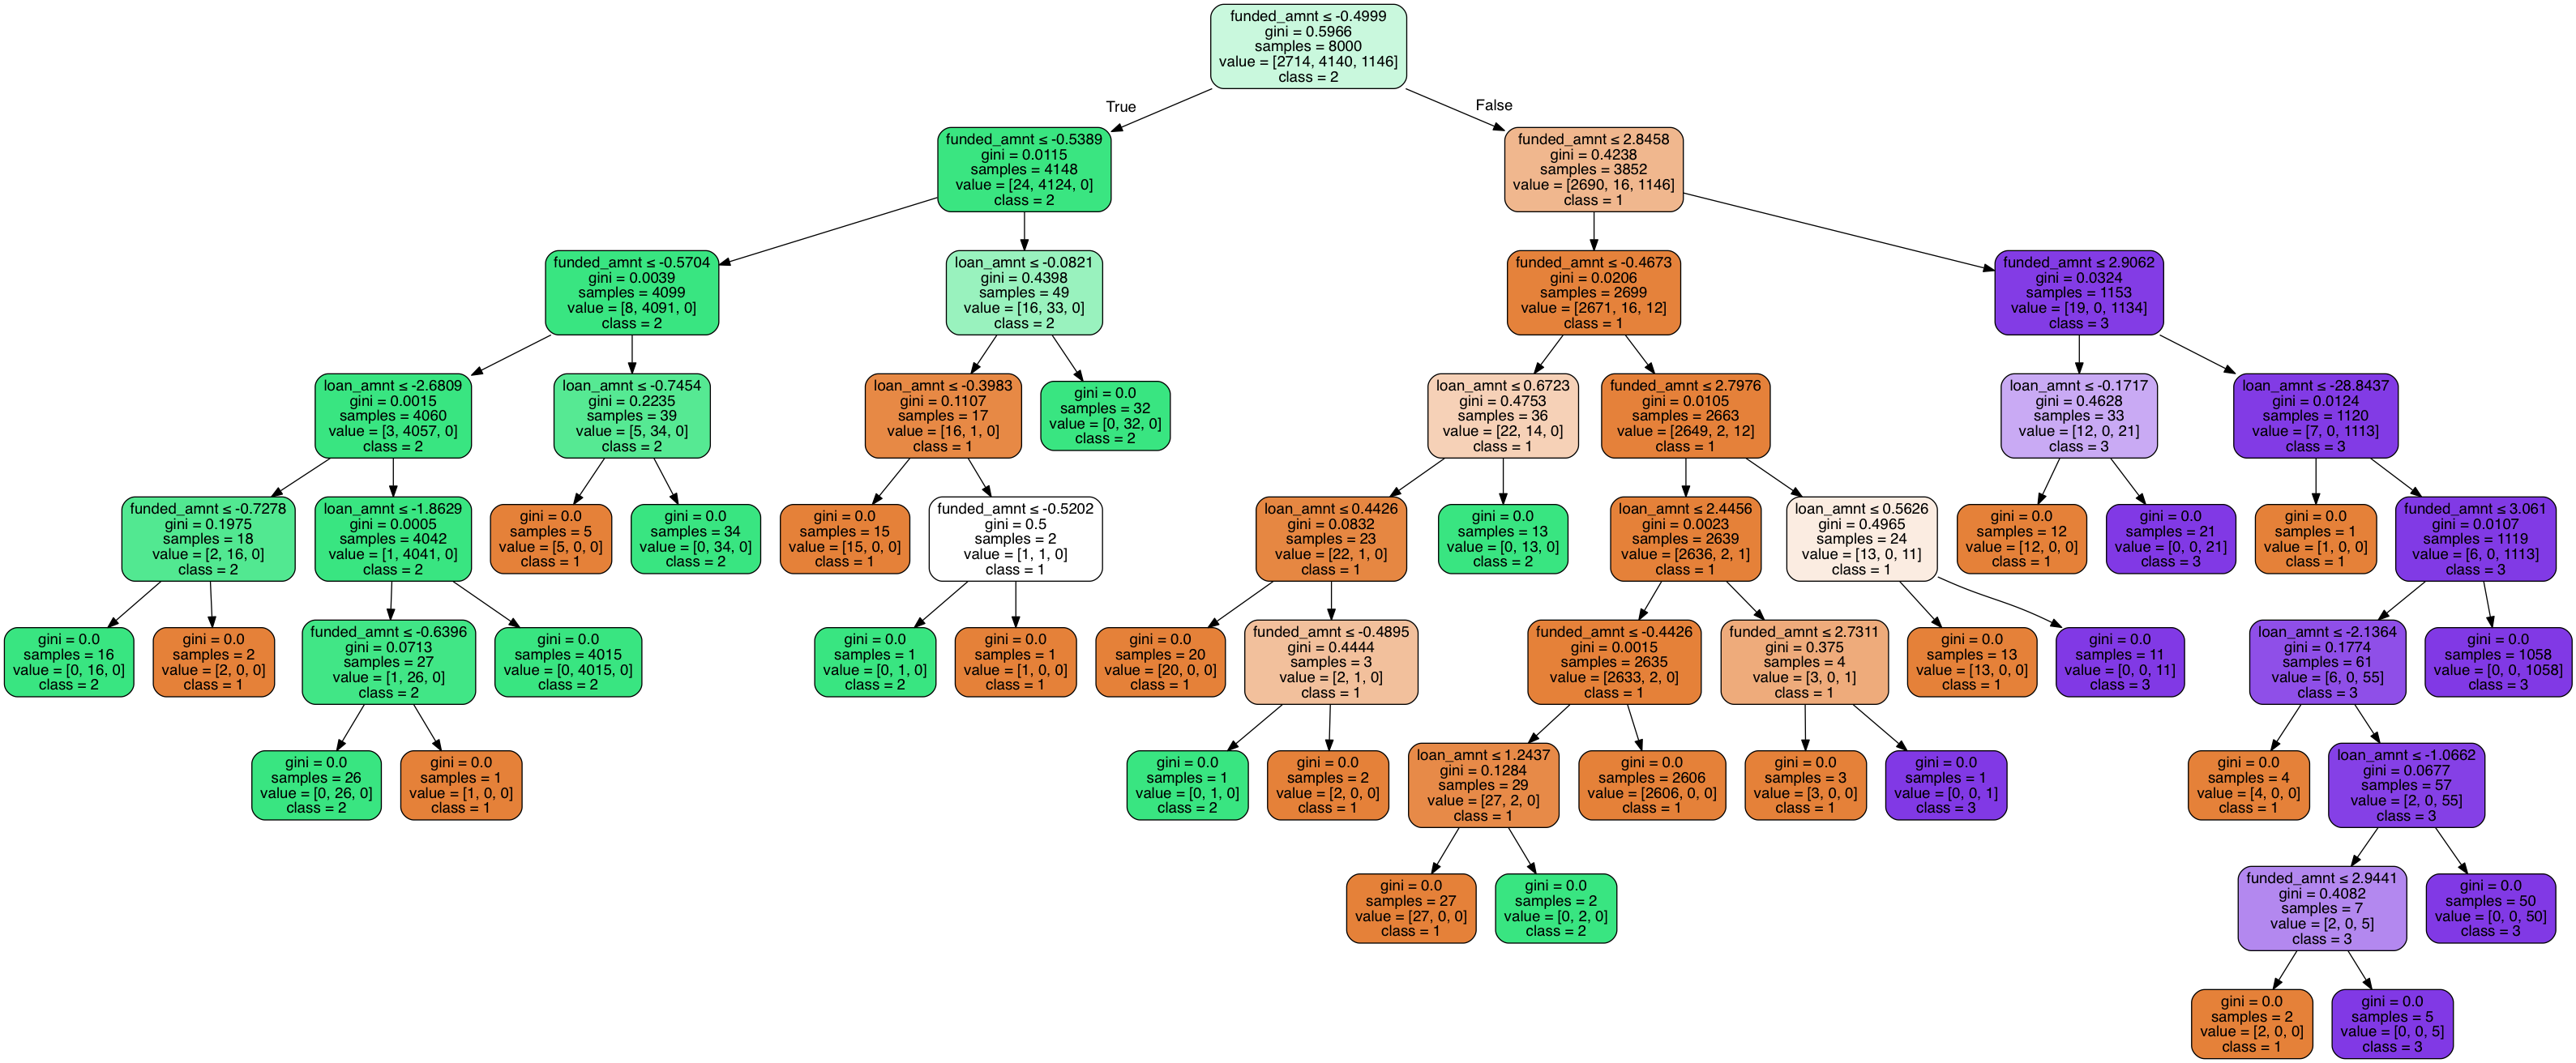
\includegraphics[width=1.05\textwidth]{img/loan}}
\fonte{Gerado a partir do script}
\end{figure}

Com este esquema, tem-se uma representação visual, de fácil interpretação de como é feito a classificação. A árvore está relativamente grande por possuir mais de 20 features. Além disso, pode ser um indício de que os dados possuem um grau de homogeneidade alto.

Ao gerar uma árvore de classificação, o algoritmo também disponibiliza a relevância das features.

\begin{figure}[!ht]
\caption{Features mais relevantes}
\centerline{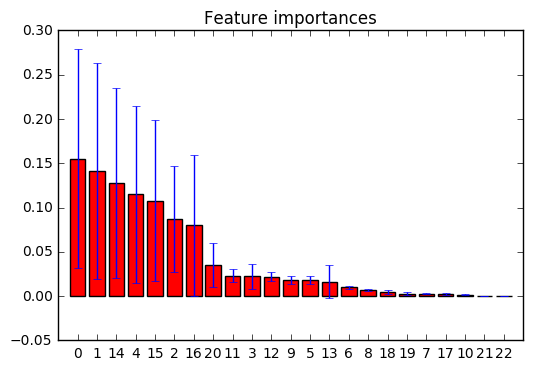
\includegraphics[width=.7\textwidth]{img/tree-most-important-features}}
\fonte{Gerado a partir do script}
\end{figure}

Desta base, é possível notar que 8 destas features possuem maior relevância frente as demais. Isso pode implicar numa redução de dimensionalidade, ocasionando economia de processamento de dados. Por outro lado, isso é válido partindo-se do pressuposto de que a natureza das informações se manterão, o que pode não ser verdade.

%
%\lstinputlisting[language=Python, firstline=37, lastline=45]{
%load_data.py
%}


\begin{figure}[!ht]
\caption{Confusion Matrix}
\centerline{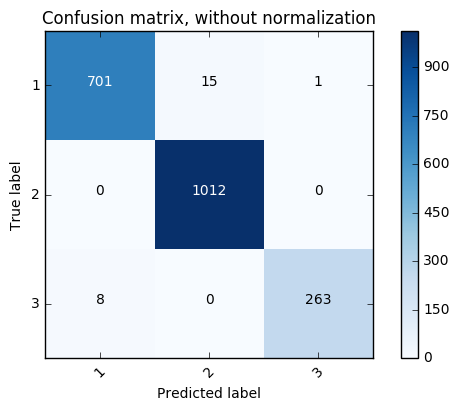
\includegraphics[width=.7\textwidth]{img/confusionMatrix}}
\fonte{Gerado a partir do script}
\end{figure}



% ---
% primeiro capitulo de Resultados
% ---
%\chapter{Lectus lobortis condimentum}
% ---

% ---
%\section{Vestibulum ante ipsum primis in faucibus orci luctus et ultrices
%posuere cubilia Curae}
% ---

%\lipsum[21-22]

% ---
% segundo capitulo de Resultados
% ---
%\chapter{Nam sed tellus sit amet lectus urna ullamcorper tristique interdum
%elementum}
% ---

% ---
%\section{Pellentesque sit amet pede ac sem eleifend consectetuer}
% ---

%\lipsum[24]

% ----------------------------------------------------------
% Finaliza a parte no bookmark do PDF
% para que se inicie o bookmark na raiz
% e adiciona espaço de parte no Sumário
% ----------------------------------------------------------
%\phantompart